\documentclass[conference]{IEEEtran}
\usepackage{amsmath,amssymb,amsfonts}
\usepackage{xcolor}
\usepackage{tikz, tikz-3dplot}
\usetikzlibrary{arrows,backgrounds,decorations,decorations.pathmorphing,
positioning,fit,automata,shapes,snakes,patterns,plotmarks,calc,trees,arrows.meta}
\usepackage{color}
\usepackage{pgfplots}
\pgfplotsset{compat=newest}
\usepackage{pgfplotstable}

\begin{document}

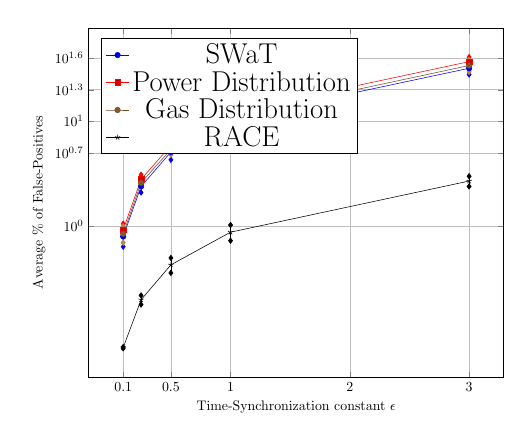
\begin{tikzpicture}[scale=0.5]
\begin{axis}[
width = \textwidth, 
grid = both, 
legend pos = north west, 
ymode = log, 
xlabel = {Time-Synchronization constant $\epsilon$}, 
ylabel={Average \% of False-Positives}, 
xtick = {0.1, 0.5, 1, 2, 3}, 
ytick = {1, 5, 10, 20, 40}, 
legend style={font=\huge}, 
bar width=0.2]

\addplot+[error bars/.cd, y dir=both, y explicit, error mark=diamond*,  error bar style={color=blue}
]
coordinates{
    (3, 32)    +-  (0, 4.1)
    (1, 10.5)    +-  (0, 1.4)
    (0.5, 5.1)    +-    (0, 0.8)
    (0.25, 2.4)   +-   (0, 0.3)
    (0.1, 0.8)    +-    (0, 0.16)
};
\addlegendentry{SWaT}

\addplot+[error bars/.cd, y dir=both, y explicit, error mark=diamond*,  error bar style={color=red}
]
coordinates{
    (3, 37)    +-  (0, 3.9)
    (1, 12.1)    +-  (0, 1.2)
    (0.5, 5.9)    +-    (0, 0.7)
    (0.25, 2.8)   +-   (0, 0.3)
    (0.1, 0.93)    +-    (0, 0.13)
};
\addlegendentry{Power Distribution}

\addplot+[error bars/.cd, y dir=both, y explicit, error mark=diamond*,  error bar style={color=brown}
]
coordinates{
    (3, 34)    +-  (0, 4.5)
    (1, 11.1)    +-  (0, 1.8)
    (0.5, 5.4)    +-    (0, 0.6)
    (0.25, 2.6)   +-   (0, 0.2)
    (0.1, 0.85)    +-    (0, 0.15)
};
\addlegendentry{Gas Distribution}

\addplot+[error bars/.cd, y dir=both, y explicit, error mark=diamond*,  error bar style={color=black}
]
coordinates{
	(3, 2.7)    +-	(0, 0.3)
    (1, 0.88)    +-	(0, 0.15)
    (0.5, 0.43)    +-	(0, 0.07)
    (0.25, 0.2)   +-	(0, 0.02)
    (0.1, 0.07)    +-	(0, 0.001)
};
\addlegendentry{RACE}

\end{axis}

\end{tikzpicture}

\end{document}